\chapter{Theoretical overview}
\label{ch:Theory}

The \textit{standard model of particle physics} (\SM{}) is an elegant attempt to describe the fundamental nature of the Universe.
At the heart of the model are the base constituents of matter, the \textit{elementary particles} and the interactions between them, the \textit{forces}.
The \SM{} describes the current experimental measurements well across a large range of energy scales.
It manages to unify forces that we can see in the macroscopic world to those binding together the constituents of protons.
The \SM{} is an incomplete model, however. 
It does not, for example, describe the gravitational interactions between particles, nor does it fully explain the matter-antimatter imbalance seen in the Universe.
Previous discrepancies in the \SM{} have lead to predictions and discoveries in Nature, such as the existence of three generations of quarks due to a lack of CP-violation observed. 
In this way, the \SM{} has evolved over the half-century since it was first postulated, to incorporate new experimental evidence to become a more complete description of nature and it will continue to do so for many years to come.
This chapter will discuss the particles which make up the \SM{} and how they interact with each other, forming the complete model.
Some drawbacks of the \SM{} will then be highlighted, before moving on to the physics of top quarks and their cross sections.

\section{The components of the standard model}
\label{sec:SM}

% Weinberg EM+W-> EWK, Glashow, Salam, Gell-mann/Zweig-> QCD
The \SM{}~\cite{Th:SM1, Th:SM2, Th:SM3, Th:SM4, Th:SM5} contains twelve types of fermion, split into leptons (\lepton{}) and quarks (\quark{}), whose interactions are mediated by four types of gauge boson.
The set of leptons exists in three generations: electrons, muons and tau particles (\electron{}, \muon{}, \tauon{}), together with their associated neutrinos, (\nue{}, \numu{}, \nutau{}). 
The set of quarks (\quark{}) also exist in three generations: up and down (\uquark{}, \dquark{}), charm and strange (\cquark{}, \squark{}) and the top and bottom (\tquark{}, \bquark{}) particles. 
For each fermion (\fermion{}) that exists there is an anti-fermion (\antifermion{}), with identical quantum properties except conjugated charges.
% Not just EM!
The properties of the fermionic particles are shown in Tab.~\ref{tb:SM_Fermions} as listed by the Particle Data Group~\cite{PDG}.
% These particles obey Fermi-Dirac statistics and are hence known as fermions. 
% $\frac{1}{e^{\frac{(\epsilon_{i}\mu)}{kT}}}$
% $\epsilon_{i}$ is the energy of the i'th state, $\mu$ is the total chemical potential
% At T=0, $\mu = E_{F}+\text{PotEnergyPerElec}$
% In a semiconductor, $\mu$ is the point of symmetry - known as the Fermi Level.
\begin{table}
	\centering
	\footnotesize
	\caption{The fermionic, spin $\sfrac{1}{2}$, particles of the \SM{} and their properties. They are split into three generations of leptons and quarks.}
	\label{tb:SM_Fermions}
	\resizebox{\linewidth}{!}{%
	\begin{tabular}{ccccccc}
								& 						& \textbf{Leptons} 			&										&						& \textbf{Quarks} 			& \\
		\vspace*{0.02cm} \textbf{Generation} 	&	\textbf{Particle} 	& \textbf{Mass (MeV)} 	& \textbf{Charge (\electron{})}			& \textbf{Particle} 	& \textbf{Mass (MeV)} 	& \textbf{Charge (\electron{})} \\
		\hline 
		1 						& \nue{}			 	& $<2\times10^{-6}$  		&	0									& \uquark{} 			& 2.2						& $\sfrac{2}{3}$ \uppertablespace\\
		 						& \electron{} 			& 0.511  					&	-1									& \dquark{} 			& 4.7						& $-\sfrac{1}{3}$ \\
		2 						& \numu{} 				& $<0.19$  					&	0									& \cquark{}	 			& 1270						& $\sfrac{2}{3}$ \\
		 						& \muon{} 		 		& 105.7	 					&	-1									& \squark{}	 			& 96						& $-\sfrac{1}{3}$ \\	
		3 						& \nutau{}	 	 		& $<18.2$  					&	0									& \tquark{}	 			& 173200					& $\sfrac{2}{3}$ \\
		 						& \tauon{}	 	 		& 1777 	 					&	-1									& \bquark{}	 			& 4180						& $-\sfrac{1}{3}$ \\	
	\end{tabular}%
	}
\end{table}

Particles in the \SM{} can interact via the electromagnetic (EM), weak and strong forces. 
In particle physics, these forces are described by quantum field theories, in which the interactions between fermions are mediated by the exchange of a virtual boson.
% Virtual is a mathematical construct combining time orderings and polarisations etc.
The EM force is mediated by the photon (\photon{}), the weak force by the massive \Wboson{} and \Zboson{} bosons and the strong force by a set of eight gluons (\gluon{}). 

The last particle of the current \SM{} is the Brout-Englert-Higgs (\BEH) boson (\Hboson), which is an excitation of the \BEH{} field.
The interaction with the \BEH{} field, via the \BEH{} mechanism, is responsible for imparting mass to the fundamental particles~\cite{Th:Higgs1, Th:Higgs2, Th:Higgs3}. 
The properties of the bosons are shown in Tab.~\ref{tb:SM_Bosons}~\cite{PDG}.
% These force mediating particles obey Bose-Einstein statistics and are hence known as Bosons.
\begin{table}
	\centering
	\footnotesize
	\caption{The bosonic, integer spin, particles of the \SM{} and their properties. The force mediators are spin 1 and the \Hboson{} boson spin 0.}
	\label{tb:SM_Bosons}
	\begin{tabular}{cccc}
		\vspace*{0.02cm} \textbf{Force Mediator} 	& \textbf{Particle} 	& \textbf{Mass (GeV)} 	& \textbf{Charge (\electron{})} \\
		\hline
		EM 							& \photon{} 			& 0 						& 0 \uppertablespace\\	 
		Weak 						& \Wboson{} 			& 80.385 					& $\pm1$ \\
									& \Zboson{}	 			& 91.188 					& 0 \\	
		Strong 						& \gluon{}				& 0 						& 0	\\	 
		---							& \Hboson{}				& 125.09 					& 0 \\	 
	\end{tabular}
\end{table}

While the \SM{} is able to describe three of the four fundamental forces between particles, it is not a complete model.
It is unable to reconcile the act of gravity at a fundamental particle level.
This is one of the discrepancies seen between the \SM{} and nature, and must be one of the future evolutions of the \SM{}.
Other problems include the baryon asymmetry seen in the Universe, the requirement for dark matter and the hierarchy problem.
These are discussed in Sec.~\ref{sec:the_full_standard_model}.

\section{Representing particles and their interactions}
\label{sec:FD}

Describing the dynamics of particles and their interactions with other particles through the excitations of relativistic quantum fields are not trivial.
To give simple visualisations of these complex interaction processes, Richard Feynman developed a powerful diagrammatic tool in 1948~\cite{Th:Feynman1, Th:Feynman2}.
This diagrammatic tool is now commonly called the Feynman diagram.
All Feynman diagrams in this thesis are created using the feyntikz package \cite{feyntikz}.
A complete Feynman diagram showing a complex example of top quark-antiquark (\ttbar{}) production and decay is shown in Fig.~\ref{fig:feyn-eg}.
In all Feynman diagrams, time increases from the left-hand side to the right, such that all the initial state particles are represented on the left and final state particles towards the right.
Each arrowed line in the Feynman diagram represents a free fermionic particle of the standard model, each sinusoidal line represents an electroweak mediator particle (\Wboson{}, \Zboson{}, \photon{}) and each coiled line a gluon.
Anti-fermions are represented as fermions moving backwards in time.
The free fermions and anti-fermions are described by the Dirac equation, which can be obtained by substituting the Lagrangian density for a Dirac field into the Euler-Lagrange equation. 
% See Appendix/,TODO.
The Lagrangian density for free fermions is given by:
\begin{equation}
\Lagr_{\text{free}}(x) = \overline{\Psi}(x)(i\gamma^{\mu}\partial_{\mu}-m)\Psi(x),
\end{equation}
where $\Psi(x)$ is the fermionic field depending on space-time, $\gamma^{\mu}$ are the gamma matrices, $\partial_{\mu}$ is the partial derivative and $m$ the fermion mass.
The $\Lagr_{\text{free}}$ is invariant under the global phase transformation,
\begin{equation}
\Psi(x) \to e^{iq\chi}\Psi(x),
\end{equation}
which is a global $\mathrm{U(1)}$ symmetry, and by Noether's theorem there must be a conserved current and charge which can be identified with the \EM{} current and charge~\cite{Th:Noether}.
When a local phase transformation is applied however,
\begin{equation}
\Psi(x) \to e^{iq\chi(x)}\Psi(x),
\end{equation}
\begin{landscape}
\begin{figure*}
\centering
\begin{resizedtikzpicture}{0.9\linewidth}
\begin{feynman}
	\vertex (i1) {\(d\)};
	\vertex [right=3cm of i1](a);
	\vertex [above right=0.75cm and 1.5cm of a] (b){ISR};
	\vertex [below right=0.75cm and 1.5cm of a] (c);

	\vertex [above=2em of i1](i1a){\(u\)};
	\vertex [above=1em of i1](i1b){\(u\)};
	\vertex [right=3cm of i1a](i1ai);
	\vertex [right=3cm of i1b](i1bi);
	\vertex [above right=0.75cm and 1.5cm of i1ai] (i1aii);
	\vertex [above right=0.75cm and 1.5cm of i1bi] (i1bii);

	\vertex [right=1cm of i1a](g1);
	\vertex [right=2cm of i1a](g2);

	\vertex [below=5em of i1](i2){\(u\)};
	\vertex [right=1.5cm of i2] (d);
	\vertex [above right=0.75cm and 1.5cm of d] (e);
	\vertex [below right=0.75cm and 1.5cm of d] (f);
	\vertex [below right=0.75cm and 1.5cm of e] (g);
	\vertex [above right=0.75cm and 1.5cm of e] (h);

	\vertex [below=1em of i2](i2a){\(u\)};
	\vertex [below=2em of i2](i2b){\(d\)};
	\vertex [right=1.5cm of i2a](i2ai);
	\vertex [right=1.5cm of i2b](i2bi);
	\vertex [below right=0.75cm and 1.5cm of i2ai] (i2aii);
	\vertex [below right=0.75cm and 1.5cm of i2bi] (i2bii);

	\vertex [right=2cm of h] (i);
	\vertex [above right=1.5cm and 1.5cm of i] (j);
	\vertex [below right=1.5cm and 1.5cm of i] (k);
	\vertex [above right=1.2cm and 1.5cm of j] (j1);
	\vertex [below right=1.2cm and 1.5cm of j] (j2);
	\vertex [above right=1.2cm and 1.5cm of k] (k1);
	\vertex [below right=1.2cm and 1.5cm of k] (k2);

	\vertex [above right=0.5cm and 1.5cm of j1] (l1){\(\ell\)};
	\vertex [below right=0.5cm and 1.5cm of j1] (l2){\(\overline \nu_\ell\)};
	\vertex [above right=0.5cm and 1.5cm of k1] (m1){\(q\)};
	\vertex [below right=0.5cm and 1.5cm of k1] (m2){\(\overline q'\)};
	\vertex [above right=0.5cm and 1.5cm of k2] (o1){\(\overline b\)};
	\vertex [below right=0.5cm and 1.5cm of k2] (o2){FSR};

	\diagram* {
	(i1) -- [fermion] (a) -- [fermion, edge label=\(q\)] (h),
	(g1) -- [gluon, half left] (g2),
	(a) -- [gluon] (b),
	(i2) -- [fermion] (d) -- [gluon] (e),
	(d) -- [fermion] (f),
	(e) -- [fermion] (g),
	(h) -- [fermion, edge label=\(\overline q\)] (e),
	(h) -- [gluon] (i),
	(i) -- [fermion, edge label=\(t\)] (j),
	(k) -- [fermion, edge label=\(\overline t\)] (i),
	(j) -- [boson, edge label=\(W^+\)] (j1),
	(j) -- [fermion, edge label=\(b\)] (j2),
	(k) -- [boson, edge label=\(W^-\)] (k1),
	(k2) -- [fermion, edge label=\(\overline b\)] (k),
	(j1) -- [fermion] (l1),
	(l2) -- [fermion] (j1),
	(k1) -- [fermion] (m1),
	(m2) -- [fermion] (k1),
	(o1) -- [fermion] (k2),
	(k2) -- [gluon] (o2),
	(i1a) -- [fermion] (i1ai) -- [fermion] (i1aii),
	(i1b) -- [fermion] (i1bi) -- [fermion] (i1bii),
	(i2a) -- [fermion] (i2ai) -- [fermion] (i2aii),
	(i2b) -- [fermion] (i2bi) -- [fermion] (i2bii),
	};
\end{feynman}
\end{resizedtikzpicture}
\caption[A Feynman diagram showing the \ttbar{} pair production by quark-anti-quark annihilation and decay into the single lepton final state (See Section\,\ref{sub:top_quark_decay}). Also shown are soft radiative processes in both the initial (ISR) and final state (FSR). Within the proton, there are also many \QCD{} interactions occuring, such that the colliding partons in the initial state are governed by the parton distribution function (See Section\,\ref{sub:top_quark_production}). All Feynman diagrams have been created using the feyntikz package.]{A Feynman diagram showing the \ttbar{} pair production by quark-anti-quark annihilation and decay into the single lepton final state (See Section\,\ref{sub:top_quark_decay}). Also shown are soft radiative processes in both the initial (ISR) and final state (FSR). Within the proton, there are also many \QCD{} interactions occuring, such that the colliding partons in the initial state are governed by the parton distribution function (See Section\,\ref{sub:top_quark_production}). All Feynman diagrams have been created using the feyntikz package \cite{feyntikz}. }
\label{fig:feyn-eg}
\end{figure*}
\end{landscape}

where the phase $q\chi(x)$ depends on space-time, the Lagrangian is no longer invariant, but contains the additional term:
\begin{equation}
\Lagr_{\text{free}}(x) = \Lagr_{\text{free}}(x)-q\overline{\Psi}(x)\gamma^{\mu}\partial_{\mu}(\chi(x))\Psi(x).
\end{equation}
This violation is solved by the introduction of a new gauge vector field, $A_{\mu}$, and coupling constant $q$ into the Lagrangian density, via the \textit{covariant derivative}
\begin{equation}
D_{\mu} = \partial_{\mu}+iqA_{\mu}.
\end{equation}
This gauge field interacts with the fermion field $\Psi$ cancelling the additional term and maintaining gauge invariance, provided the photon field is massless.
The combination of the free fermionic fields, photon fields and the EM interaction term is known as \textit{Quantum Electrodynamics} (\QED{}), with the full Lagrangian density given as:
\begin{equation}
\Lagr_{\mathrm{QED}}=\overline{\Psi}(i\gamma^{\mu}\partial_{\mu}-m)\Psi - \frac{1}{4}F^{\mu \nu }F_{\mu \nu } + q\overline{\Psi}\gamma^{\mu}\Psi A_{\mu},
\end{equation}
where $F^{\mu \nu}$ is the EM field strength tensor with the term describing free photons.
% ASIDE SEE APP
% U(1) The generator is a 1x1 matrix (theta)

\section{Quantum chromodynamics}
\label{sec:QCD}

The quantum field theory for the strong interaction, \textit{Quantum Chromodynamics} (\QCD{}), is similar in many ways to that of \QED{}.
The strong interactions are highlighted in red on Fig.~\ref{fig:feyn-qcd}.
\begin{figure}[h!]
\centering
\begin{tikzpicture}
\begin{feynman}
	\vertex [red!50](i1){\(d\)};
	\vertex [red!50,right=3cm of i1](a);
	\vertex [red!50,above right=0.75cm and 1.5cm of a] (b){ISR};
	\vertex [red!50,below right=0.75cm and 1.5cm of a] (c);

	\vertex [red!50,above=2em of i1](i1a){\(u\)};
	\vertex [red!50,above=1em of i1](i1b){\(u\)};
	\vertex [black!50,right=3cm of i1a](i1ai);
	\vertex [black!50,right=3cm of i1b](i1bi);
	\vertex [black!50,above right=0.75cm and 1.5cm of i1ai] (i1aii);
	\vertex [black!50,above right=0.75cm and 1.5cm of i1bi] (i1bii);

	\vertex [right=1cm of i1a](g1);
	\vertex [right=2cm of i1a](g2);

	\vertex [red!50,below=5em of i1](i2){\(u\)};
	\vertex [red!50,right=1.5cm of i2] (d);
	\vertex [red!50,above right=0.75cm and 1.5cm of d] (e);
	\vertex [red!50,below right=0.75cm and 1.5cm of d] (f);
	\vertex [red!50,below right=0.75cm and 1.5cm of e] (g);
	\vertex [red!50,above right=0.75cm and 1.5cm of e] (h);

	\vertex [red!50,below=1em of i2](i2a){\(u\)};
	\vertex [red!50,below=2em of i2](i2b){\(d\)};
	\vertex [black!50,right=1.5cm of i2a](i2ai);
	\vertex [black!50,right=1.5cm of i2b](i2bi);
	\vertex [black!50,below right=0.75cm and 1.5cm of i2ai] (i2aii);
	\vertex [black!50,below right=0.75cm and 1.5cm of i2bi] (i2bii);

	\vertex [red!50,right=2cm of h] (i);
	\vertex [red!50,above right=1.5cm and 1.5cm of i] (j);
	\vertex [red!50,below right=1.5cm and 1.5cm of i] (k);
	\vertex [red!50,above right=1.2cm and 1.5cm of j] (j1);
	\vertex [red!50,below right=1.2cm and 1.5cm of j] (j2);
	\vertex [red!50,above right=1.2cm and 1.5cm of k] (k1);
	\vertex [red!50,below right=1.2cm and 1.5cm of k] (k2);

	\vertex [black!50,above right=0.5cm and 1.5cm of j1] (l1){\(\ell\)};
	\vertex [black!50,below right=0.5cm and 1.5cm of j1] (l2){\(\overline \nu_\ell\)};
	\vertex [black!50,above right=0.5cm and 1.5cm of k1] (m1){\(q\)};
	\vertex [black!50,below right=0.5cm and 1.5cm of k1] (m2){\(\overline q'\)};
	\vertex [red!50,above right=0.5cm and 1.5cm of k2] (o1){\(\overline b\)};
	\vertex [red!50,below right=0.5cm and 1.5cm of k2] (o2){FSR};

	\diagram* {
	(i1) -- [red!50,fermion] (a) -- [red!50,fermion, edge label=\(q\)] (h),
	(g1) -- [red!50,gluon, half left] (g2),
	(a) -- [red!50,gluon] (b),
	(i2) -- [red!50,fermion] (d) -- [red!50,gluon] (e),
	(d) -- [red!50,fermion] (f),
	(e) -- [red!50,fermion] (g),
	(h) -- [red!50,fermion, edge label=\(\overline q\)] (e),
	(h) -- [very thick,red,gluon] (i),
	(i) -- [very thick,red,fermion, edge label=\(t\)] (j),
	(k) -- [very thick,red,fermion, edge label=\(\overline t\)] (i),
	(j) -- [black!50,boson, edge label=\(W^+\)] (j1),
	(j) -- [black!50,fermion, edge label=\(b\)] (j2),
	(k) -- [black!50,boson, edge label=\(W^-\)] (k1),
	(k2) -- [red!50,fermion, edge label=\(\overline b\)] (k),
	(j1) -- [black!50,fermion] (l1),
	(l2) -- [black!50,fermion] (j1),
	(k1) -- [black!50,fermion] (m1),
	(m2) -- [black!50,fermion] (k1),
	(o1) -- [red!50,fermion] (k2),
	(k2) -- [red!50,gluon] (o2),
	(i1a) -- [red!50,fermion] (i1ai) -- [red!50,fermion] (i1aii),
	(i1b) -- [red!50,fermion] (i1bi) -- [red!50,fermion] (i1bii),
	(i2a) -- [red!50,fermion] (i2ai) -- [red!50,fermion] (i2aii),
	(i2b) -- [red!50,fermion] (i2bi) -- [red!50,fermion] (i2bii),
	};
\end{feynman}
\end{tikzpicture}
\caption[A Feynman diagram showing the \ttbar{} pair production and decay. An example QCD interaction is shown in bold red. Other QCD interactions are shown in light red.]{A Feynman diagram showing the \ttbar{} pair production and decay. An example QCD interaction is shown in bold red. Other QCD interactions are shown in light red.}
\label{fig:feyn-qcd}
\end{figure}
It is described by an $\mathrm{SU(3)}$ symmetry group, with three orthogonal states known as colour charges ($r,g,b$).
To maintain invariance under the local $\mathrm{SU(3)}$ gauge transformation
\begin{equation}
\Psi(x) \to e^{i\theta^{a}(x)t^{a}}\Psi(x),
\end{equation}
eight new gauge fields, $G_{\mu}^{a}$, must be introduced in a similar manner to \QED{}.
These fields come from the eight generators of the $\mathrm{SU(3)}$ symmetry group $t^{a}$, which can be represented by the Gell-Mann matrices as $t^{a}=-\frac{1}{2}\lambda^{a}$.
As with \QED{}, the extra fields are folded into the covariant derivative, this time with a strong coupling constant $g_{s}$
\begin{equation}
D_{\mu} = \partial_{\mu}+ig_{s}\frac{\lambda_{a}}{2}G_{\mu}^{a}.
\end{equation}
Thus the strong force is mediated by eight massless gauge bosons (gluons), however, in difference to \QED{}, these gluons carry a colour charge brought about by the non-commutation of the $\mathrm{SU(3)}$ generators, leading to gluon-gluon self-interactions.
The full \QCD{} Lagrangian density is given as
\begin{equation}
\Lagr_{\QCD}=\overline{\Psi}_{i}([i\gamma^{\mu}D_{\mu}]_{ij}-m\delta_{ij})\Psi_{j} - \frac{1}{4}G^{\mu \nu}_{a}G^{a}_{\mu \nu},
\end{equation}
where the gluon field strength tensor 
\begin{equation}
	G_{\mu \nu}^{a}=\partial_{\mu}G_{\nu}^{a} - \partial_{\nu}G_{\mu}^{a} + g_{s}f^{abc}G_{\mu}^{b}G_{\nu }^{c},
\end{equation}
is analogous to the electromagnetic field strength tensor and the $\mathrm{SU(3)}$ fine structure constants $f^{abc}$, are introduced by the gluon-gluon self-interaction.

\subsection{Colour confinement and hadronisation} % (fold)
\label{sub:confinement}
In Fig.~\ref{fig:alphaSrunning}, the running of the strong coupling constant with energy is shown.
\begin{figure}[h!]
	\centering
	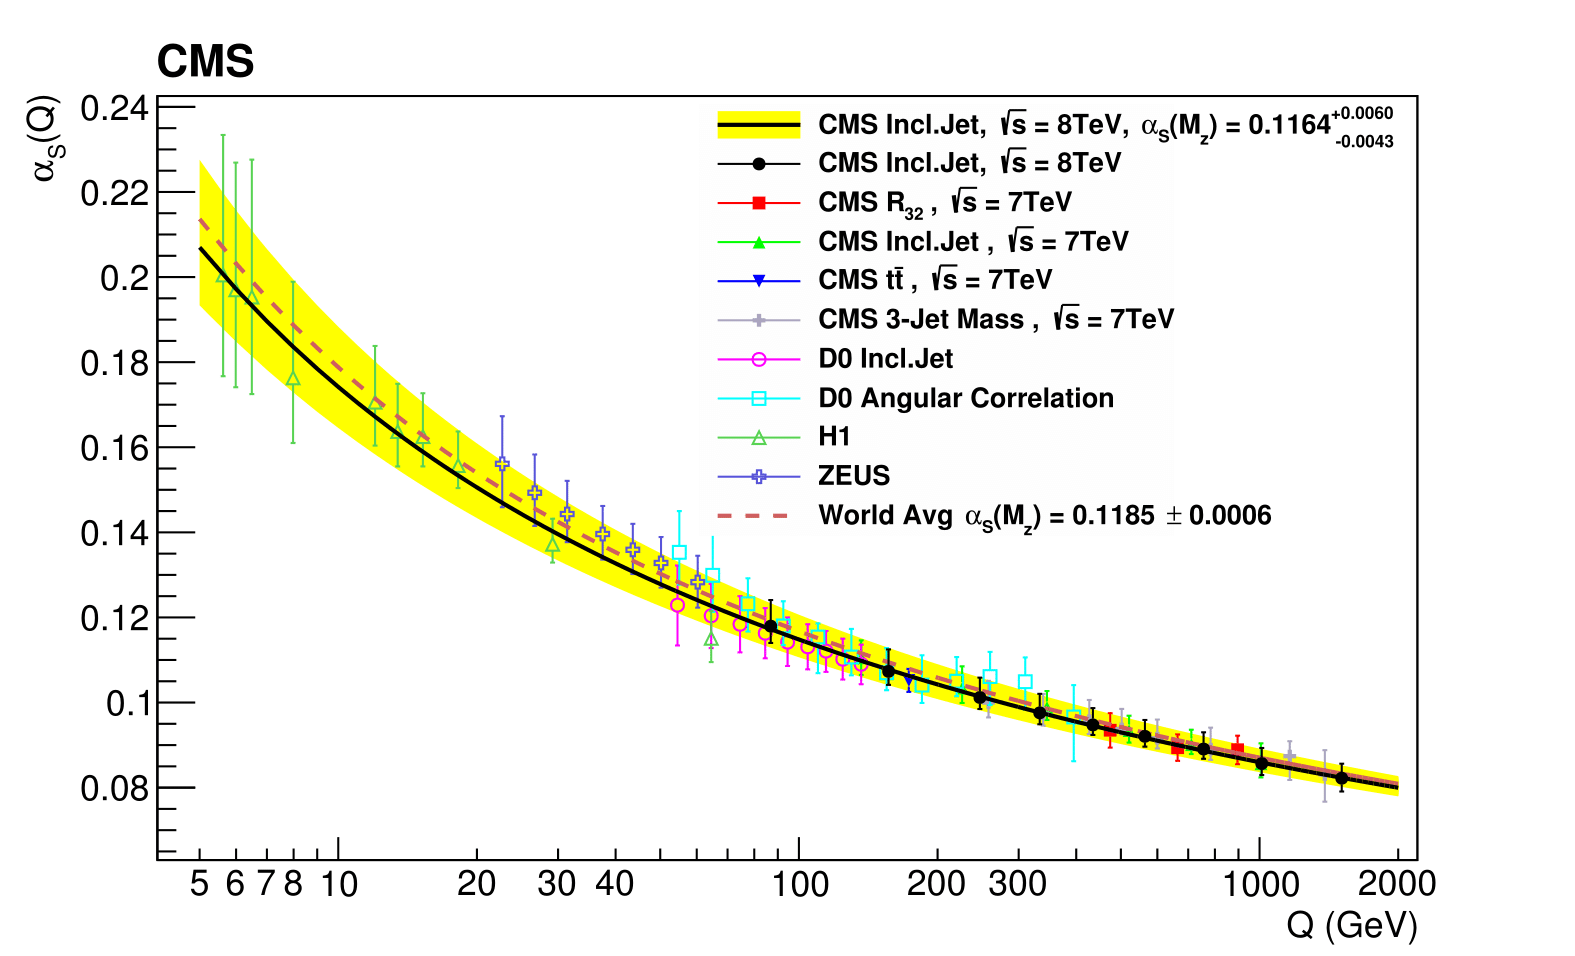
\includegraphics[width=\textwidth]{Figures/alphaS}
	\caption[The running of the strong coupling constant. At higher energy scales \alpS{} tends to 0, resulting in a strengthening of the strong force.]{The running of the strong coupling constant. At higher energy scales \alpS{} tends to 0, resulting in a strengthening of the strong force. \cite{alphaSrunning}.}
	\label{fig:alphaSrunning}
\end{figure}
At higher energies the strong coupling constant $g_{s}$ (or $\alpS = \sfrac{g_{s}^{2}}{4\pi}$) tends to 0.
This is known as asymptotic freedom and means that the strong force becomes stronger at larger quark or gluon separations.
The quarks and gluons are consequently bound in colourless states (hadrons and mesons) in a process known as \textit{colour confinement}.
Single quarks in the final state of Fig.~\ref{fig:feyn-eg} bind into baryons within a time scale of $\tau_{\mathrm{had}} \simeq \sfrac{1}{\Lambda_{\mathrm{QCD}}} \approx 3\ten{-24}\s$.
These particles can be highly energetic and if the potential energy due to the strong force confining a \qqbar{} pair is large enough then a new \qqbar{} pair will be produced from the vacuum. 
If the new daughter hadrons produced also have enough energy, the process is repeated until the confinement is strong enough to hold them together.
The splitting of hadrons and mesons in this way is known as \textit{hadronisation} and results in a spray of particles known in experimental terms as a \textit{jet}.
Similarly, when a hard interaction occurs within the colliding protons, the protons cease to become colourless states, and the remnants hadronise forming more sprays of particles.
These particles are known as the \textit{underlying event}.
The hadronisation process will be discussed in more detail in Sec.~\ref{sec:fragmentation_and_colour_reconnection}.
% subsection confinement (end)



\section{The weak interaction and electroweak unification}
\label{sec:EWK}

The weak interaction differs from \QED{} and \QCD{} in that it is possible to violate parity conservation $\Psi(x)\neq\Psi(-x)$, and to change the flavour of a quark. 
% It is also mediated by three massive gauge bosons.
Example weak interactions are highlighted in blue on Fig.~\ref{fig:feyn-ewk}.
The weak interaction is described by an $\mathrm{SU(2)}$ symmetry group, with the conserved charge being the weak isospin $T$.
The third component of weak isospin $T_{3}$, is also conserved.
Parity violation is seen in the weak interaction as only left-handed particles and right-handed anti-particles have been observed to interact via the weak force. 
% Left handed particles are particle s in which the spin directio is opposite the directio of motion
% This leads to the assumption that neutrinos are massless
\begin{figure}[h!]
\centering
\begin{tikzpicture}
\begin{feynman}
	\vertex [black!50](i1) {\(d\)};
	\vertex [right=3cm of i1](a);
	\vertex [black!50,above right=0.75cm and 1.5cm of a] (b){ISR};
	\vertex [below right=0.75cm and 1.5cm of a] (c);

	\vertex [black!50,above=2em of i1](i1a){\(u\)};
	\vertex [black!50,above=1em of i1](i1b){\(u\)};
	\vertex [right=3cm of i1a](i1ai);
	\vertex [right=3cm of i1b](i1bi);
	\vertex [above right=0.75cm and 1.5cm of i1ai] (i1aii);
	\vertex [above right=0.75cm and 1.5cm of i1bi] (i1bii);

	\vertex [right=1cm of i1a](g1);
	\vertex [right=2cm of i1a](g2);

	\vertex [black!50,below=5em of i1](i2){\(u\)};
	\vertex [right=1.5cm of i2] (d);
	\vertex [above right=0.75cm and 1.5cm of d] (e);
	\vertex [below right=0.75cm and 1.5cm of d] (f);
	\vertex [below right=0.75cm and 1.5cm of e] (g);
	\vertex [above right=0.75cm and 1.5cm of e] (h);

	\vertex [black!50,below=1em of i2](i2a){\(u\)};
	\vertex [black!50,below=2em of i2](i2b){\(d\)};
	\vertex [right=1.5cm of i2a](i2ai);
	\vertex [right=1.5cm of i2b](i2bi);
	\vertex [below right=0.75cm and 1.5cm of i2ai] (i2aii);
	\vertex [below right=0.75cm and 1.5cm of i2bi] (i2bii);

	\vertex [right=2cm of h] (i);
	\vertex [above right=1.5cm and 1.5cm of i] (j);
	\vertex [below right=1.5cm and 1.5cm of i] (k);
	\vertex [above right=1.2cm and 1.5cm of j] (j1);
	\vertex [below right=1.2cm and 1.5cm of j] (j2);
	\vertex [above right=1.2cm and 1.5cm of k] (k1);
	\vertex [below right=1.2cm and 1.5cm of k] (k2);

	\vertex [blue!50,above right=0.5cm and 1.5cm of j1] (l1){\(\ell\)};
	\vertex [blue!50,below right=0.5cm and 1.5cm of j1] (l2){\(\overline \nu_\ell\)};
	\vertex [blue!50,above right=0.5cm and 1.5cm of k1] (m1){\(q\)};
	\vertex [blue!50,below right=0.5cm and 1.5cm of k1] (m2){\(\overline q'\)};
	\vertex [black!50,above right=0.5cm and 1.5cm of k2] (o1){\(\overline b\)};
	\vertex [black!50,below right=0.5cm and 1.5cm of k2] (o2){FSR};

	\diagram* {
	(i1) -- [black!50,fermion] (a) -- [black!50,fermion, edge label=\(q\)] (h),
	(g1) -- [black!50,gluon, half left] (g2),
	(a) -- [black!50,gluon] (b),
	(i2) -- [black!50,fermion] (d) -- [black!50,gluon] (e),
	(d) -- [black!50,fermion] (f),
	(e) -- [black!50,fermion] (g),
	(h) -- [black!50,fermion, edge label=\(\overline q\)] (e),
	(h) -- [black!50,gluon] (i),
	(i) -- [blue,very thick,fermion, edge label=\(t\)] (j),
	(k) -- [blue!50,fermion, edge label=\(\overline t\)] (i),
	(j) -- [blue,very thick,boson, edge label=\(W^+\)] (j1),
	(j) -- [blue,very thick,fermion, edge label=\(b\)] (j2),
	(k) -- [blue!50,boson, edge label=\(W^-\)] (k1),
	(k2) -- [blue!50,fermion, edge label=\(\overline b\)] (k),
	(j1) -- [blue!50,fermion] (l1),
	(l2) -- [blue!50,fermion] (j1),
	(k1) -- [blue!50,fermion] (m1),
	(m2) -- [blue!50,fermion] (k1),
	(o1) -- [black!50,fermion] (k2),
	(k2) -- [black!50,gluon] (o2),
	(i1a) -- [black!50,fermion] (i1ai) -- [black!50,fermion] (i1aii),
	(i1b) -- [black!50,fermion] (i1bi) -- [black!50,fermion] (i1bii),
	(i2a) -- [black!50,fermion] (i2ai) -- [black!50,fermion] (i2aii),
	(i2b) -- [black!50,fermion] (i2bi) -- [black!50,fermion] (i2bii),
	};
\end{feynman}
\end{tikzpicture}
\caption[A Feynman diagram showing the \ttbar{} pair production and decay. An example weak interaction is shown in bold blue. Other weak interactions are shown in light blue.]{A Feynman diagram showing the \ttbar{} pair production and decay. An example weak interaction is shown in bold blue. Other weak interactions are shown in light blue.}
\label{fig:feyn-ewk}
\end{figure}
% approx 100GeV
% Y = 2(q-I3)
At higher energies, the electromagnetic and weak interactions unify into the electroweak (\EWK{}) interaction.
This combination results in a \ensuremath{\mathrm{SU(2)_{L}}\otimes\mathrm{U(1)_{Y}}} symmetry group, with three gauge fields, $W^{i}_{\mu}$, introduced by the $\mathrm{SU(2)_{L}}$ generators $\frac{1}{2}\sigma_{i}$ (the Pauli spin matrices) and one gauge field, $B_{\mu}$, from the $\mathrm{U(1)_{Y}}$ generator (weak hypercharge $Y = 2(Q-T_{3})$).
% Fermions with negative chirality (also called “left-handed” fermions) have T = 1/2, T3 pm1/2.
% Group into doublets (u, d)->(ve, e)->(1/2, -1/2)
% Behave similarly under weak interactions
% Never decays weakly into particle of the same T3.
% The corresponding anti-fermion has reversed chirality (“right-handed” antifermion) and sign reversed T3.
% Fermions with positive chirality (“right-handed” fermions) and anti-fermions with negative chirality (“left-handed” anti-fermions) have T3=0
% Form singlets that do not undergo weak interactions.
The \EWK{} gauge bosons are formed from the interferences of these fields and are formed as:
\begin{equation}
	W^{\pm}_{\mu} = \frac{1}{\sqrt{2}}(W^{1}_{\mu} \mp iW^{2}_{\mu}),
\end{equation}
\begin{equation}
	Z_{\mu} = W^{3}_{\mu}\cos{\theta_{W}} -  B_{\mu}\sin{\theta_{W}},
\end{equation}
and 
\begin{equation}
	A_{\mu} = W^{3}_{\mu}\sin{\theta_{W}} +  B_{\mu}\cos{\theta_{W}},
\end{equation}
% 4DOUG essentially four fields are created... two charged and two neutral. This fields interfere and the excitations of these inteferences give the gauge bosons.
where $\theta_{W}$ is the weak mixing angle~\cite{Th:SM1}, defined by the ratio of the two weak coupling constants (isospin and isocharge) 
\begin{equation}
	\tan(\theta_{W}) = \frac{g'}{g_{W}}.	
\end{equation}
The full \EWK{} covariant derivative and Lagrangian density are given by
\begin{equation}
D_{\mu} = \partial_{\mu}+ig_{W}\frac{\sigma_{i}}{2}W_{\mu}^{i}+ig'\frac{Y_{W}}{2}B_{\mu},
\end{equation}
and
\begin{equation}
\Lagr_{\EWK}=\overline{\Psi}i\gamma^{\mu}D_{\mu}\Psi - \frac{1}{4}B^{\mu\nu}B_{\mu\nu} - \frac{1}{4}W^{\mu\nu}_{i}W_{\mu\nu}^{i},
\end{equation}
respectively.
If this is assumed to be an accurate representation of the \EWK{} interaction, it requires that gauge bosons and fermions be massless in order to preserve the gauge symmetry.
As it is experimentally proven that fermions and the \Wboson{} and \Zboson{} bosons have mass, a solution is needed.
The problem is solved through a process called \textit{electroweak symmetry breaking}.

\subsection{Electroweak symmetry breaking} % (fold)
\label{sub:electroweak_symmetry_breaking}

Electroweak symmetry breaking solves the mass problem by keeping the particles massless but introducing a new complex scalar field doublet and potential into the Lagrangian density.
% 4 degrees of freedom - three to give mass to weak bosons
% The Higgs mechanism can be summarized by saying that the spontaneous breaking of a gauge theory by a non-zero VEV results in the disappearance of a Goldstone boson and its transformation into the longitudinal component of a massive gauge boson.
% Scalar VEV does not affect electromagnetism
% \begin{equation}
% 	\phi = 	\phi_1+i\phi_2 \\
% \end{equation}
\begin{equation}
	\phi = 
\begin{pmatrix} 
	\phi^{+} \\
	\phi^{0} \\
\end{pmatrix}
	= 
\begin{pmatrix} 
	\phi_1+i\phi_2 \\
	\phi_3+i\phi_4 \\
\end{pmatrix}
\end{equation}
\begin{equation}
\Lagr_{\mathrm{H}}=(D_{\mu}\phi)^{\dagger}(D^{\mu}\phi)-\frac{1}{2}\mu^{2}\phi^{\dagger}\phi - \frac{1}{4}\lambda(\phi^{\dagger}\phi)^{2}
\end{equation}
This potential introduces an infinite set of degenerate non-zero ground states of $\phi$.
The vacuum expectation value $v$, is the magnitude of an arbitrary ground state provided $\mu^{2}$ is negative
\begin{equation}
	v=\sqrt{-\frac{\mu^2}{\lambda}}\approx246\GeV.
\end{equation} 
The choice of $v$, conventionally along the neutral, real component of $\phi$, \textit{spontaneously} breaks the symmetry of the Lagrangian~\cite{PDG}.
The neutral component is chosen because the charged component of $\phi$ must be set to zero such that the addition of a vacuum expectation value will not break the conservation of electric charge.
By taking this choice, $\phi$ can be rewritten as a perturbation around this point
\begin{equation}
	\phi = \frac{1}{\sqrt{2}}
\begin{pmatrix} 
	0 \\
	v + H(x) \\
\end{pmatrix},
\end{equation}
where $H(x)$ is the massive \BEH{} scalar field with
\begin{equation}
	m_{H} = v\sqrt{2\lambda}.
\end{equation}
The other three degrees of freedom from the initial scalar field doublet form the three massive weak bosons, via the \BEH{} mechanism~\cite{Th:Higgs1, Th:Higgs2, Th:Higgs3} such that:
%  (\textit{Goldstone bosons})
% The longitudinal polarization components of the W and Z bosons correspond to the Goldstone bosons of the spontaneously broken part of the electroweak symmetry SU(2)⊗U(1), which, however, are not observable. 
% Because this symmetry is gauged, the three would-be Goldstone bosons are "eaten" by the three gauge bosons corresponding to the three broken generators; this gives these three gauge bosons a mass, and the associated necessary third polarization degree of freedom. This is described in the Standard Model through the Higgs mechanism.
% The Higgs mechanism is the choice of unitary gauge that 'eats' the Goldstone bosons
% Gauge symmetries do not give goldstone bosonsl they give massive bosons. Normal symmetries do.
\begin{equation}
	m_{W} = \frac{vg_{W}}{2},
	\,\,\,
	m_{Z} = \frac{v\sqrt{g_{W}^{2}+g'^{2}}}{2}.
\end{equation}
Fermions may also be permitted mass via the Higgs mechanism, by introducing additional terms to the Lagrangian density of the form 
\begin{equation} \label{eq:LY}
	\Lagr_{\mathrm{Y}} = g_{y}(\overline{\Psi}_L\phi\Psi_R+\overline{\Psi}_R\phi^{\dagger}\Psi_L), 
\end{equation}
where $g_{y}$ (\textit{Yukawa coupling}) is the coupling strength of the respective fermion to the \BEH{} field.
The Yukawa coupling strength is different for each fermion.
This leads to fermion masses which are linearly proportional to and only dependent on $g_{y}$, given by
\begin{equation}
	m_{f}=\frac{vg_{y}}{\sqrt{2}}.
\end{equation}
% subsection electroweak_symmetry_breaking (end)

\subsection{The Cabbibo-Kobayashi-Maskawa mixing matrix} % (fold)
\label{sub:the_cabbibo_kobayashi_maskawa_mixing_matrix}
The weak interaction of quarks is described by the Cabbibo-Kobayashi-Maskawa (\CKM{}) mixing matrix~\cite{Th:CKM1, Th:CKM2}.
It postulated the existence of a third family of quarks (\tquark{}, \bquark{}) to explain the observed CP violation in kaon decays~\cite{Th:CKM2}.
It relates the weak, flavour eigenstates to the mass eigenstates by
\begin{equation*}
\begin{pmatrix}
\dquark' \\
\squark' \\
\bquark'
\end{pmatrix}
=
\begin{pmatrix}
V_{\uquark\dquark} & V_{\uquark\squark} & V_{\uquark\bquark} \\
V_{\cquark\dquark} & V_{\cquark\squark} & V_{\cquark\bquark} \\
V_{\tquark\dquark} & V_{\tquark\squark} & V_{\tquark\bquark}
\end{pmatrix}
\begin{pmatrix}
\dquark \\
\squark \\
\bquark
\end{pmatrix}.
\end{equation*}
The relative strength of the weak interaction involving a flavour transition from $j\rightarrow i$ is given by the associated \CKM{} matrix element $V_{ij}$.
In the \SM{} the \CKM{} matrix is unitary ($V^{\dag}V=I$) so that each row behaves as $\abs{V_{\uquark\dquark}}^2 + \abs{V_{\uquark\squark}}^2 + \abs{V_{\uquark\bquark}}^2 = 1$.
This unitarity assumption leads to current experimental measurements of
\begin{equation*}
\begin{pmatrix}
\abs{V_{\uquark\dquark}} & \abs{V_{\uquark\squark}} & \abs{V_{\uquark\bquark}} \\
\abs{V_{\cquark\dquark}} & \abs{V_{\cquark\squark}} & \abs{V_{\cquark\bquark}} \\
\abs{V_{\tquark\dquark}} & \abs{V_{\tquark\squark}} & \abs{V_{\tquark\bquark}}
\end{pmatrix}
\approx
\begin{pmatrix}
0.974 & 0.225 & 0.004 \\
0.225 & 0.973 & 0.041 \\
0.009 & 0.040 & 0.999
\end{pmatrix},
\end{equation*}
given by~\cite{PDG}.
The relative strength of the off-diagonal \CKM{} elements means that flavour transitions between different generations of quarks are suppressed.
There is a small complex phase that is present in the $V_{\uquark\bquark}$ and $V_{\tquark\dquark}$ matrix elements, which allows for a small quantity of charge-parity (CP) violation in the \SM{}.

% Measurements senstitive to amplitude squared are not senstive to weak complex phase.
% Need measurements senstive to amplitude
% These are in neutral B and K systems.
% Use oscillations and interfereing final states.
% subsection the_cabbibo_kobayashi_maskawa_mixing_matrix (end)



\section{The standard model and its shortcomings} % (fold)
\label{sec:the_full_standard_model}
The full \SM{} combines the \QCD{} and \EWK{} field theories into the combined symmetry group \ensuremath{\mathrm{SU(3)_{c}}\otimes\mathrm{SU(2)_{L}}\otimes\mathrm{U(1)_{Y}}}.
This has the effect of making the full covariant derivative
\begin{equation}
	D_{\mu} = \partial_{\mu}+ig_{S}\frac{\lambda_{a}}{2}G_{a}+ig_{W}\frac{\sigma_{i}}{2}W_{\mu}^{i}+ig'\frac{Y_{W}}{2}B_{\mu},
\end{equation}
and the full Lagrangian density the sum of all individual components
\begin{equation}
	\Lagr_{\SM} = \Lagr_{\QCD} + \Lagr_{\EWK} + \Lagr_{\mathrm{H}} + \Lagr_{\mathrm{Y}}.
\end{equation}
It includes terms for free fermions and gauge bosons and the interactions between them, in addition to mass terms arising from the introduction of the \BEH{} field and a non-zero $v$.
It is the most complete model we have of our Universe, describing fundamental matter and its interactions to an unprecedented degree of precision, however as mentioned earlier, it is far from a complete description.
% section the_full_standard_model (end)

\subsection{Gravity} % (fold)
\label{sub:gravity}

Perhaps the largest omission from the \SM{} is the fundamental force of gravity, which all massive particles experience.
In order to include a description of gravity in the \SM{}, a unification with the theory of general relativity at the quantum scale is needed.
The formulation of this unification at present is unknown, however one popular way to do this is with string theory.
Unfortunately, the effect of gravity is completely negligible at the current accessible energy scales and as such it is not experimentally feasible to directly test any unification theory.  
% $\Lamdba_{P} \sim \ten{19} \GeV$
% subsection gravity (end)

\subsection{Massive neutrinos} % (fold)
\label{sub:massive_neutrinos}

The current observation that only left-handed neutrinos interact weakly results in the Yukawa component of the Lagrangian density shown in Eq.~\ref{eq:LY}, losing gauge invariance unless the neutrinos are massless.
Experiments such as SNO which measured a third of the number of \nue{} expected from production in the Sun~\cite{Th:SNO}, or Super-Kamiokande which measured half of the number of upward atmospheric \numu{} as downward ones~\cite{Th:SuperK}, prove an oscillation in the flavour of the neutrino.
This can be explained by the neutrinos acquiring a mass, such that the flavour states of the neutrinos are then linear superpositions of the mass states.
% Removing this statement as i don't like it - nor do i want to talk about it
% There is also no reason why right-handed neutrinos should not exist in nature.
% Goldhaber Experiment? https://indico.cern.ch/event/73981/contributions/2080329/attachments/1043729/1487656/Grodzins_Lee_Monday_Opening.pdf 
% subsection massive_neutrinos (end)

\subsection{Dark matter} % (fold)
\label{sub:dark_matter}

Other issues with the \SM{} originate from cosmological observations.
Firstly, the lack of enough mass in galaxies to explain the rotation curves of luminous matter, provides evidence for a type of additional matter which must be massive and electromagnetically inert~\cite{Th:DM1}.
This matter is known as dark matter and is predicted to contribute around 80\% to the matter content of the Universe. 
There are other cosmological indicators for dark matter including galaxy clusters~\cite{Th:DM2} and the cosmic microwave background~\cite{Th:DM3}.
While the current \SM{} does provide a set of particles which behave in this way, the neutrinos, there are not enough to account for all of the missing matter and they are too 'hot`, \ie{} their highly relativistic velocity is unable to explain observations.

The second issue is that the observation of the accelerating expansion of the Universe implies that there is a repulsive operation acting~\cite{Th:DM4}.
This process is enshrined under the term dark energy, which accounts for 70\% of the mass-energy content of the Universe.
The \SM{} has no mechanism for describing dark energy.
% Clusters: Viral theorem (essentially roation curve again) and lensing 
% CMB: anisotropy can be mapped to power law spectrum. three peaks.. 3rd relates to DM.
% subsection dark_matter (end)

\subsection{Baryon asymmetry} % (fold)
\label{sub:baryon_asymmetry}

Another striking problem in the \SM{} is the matter-antimatter imbalance seen in the Universe.
The Universe is predominantly matter based, however the \SM{} predicts that matter and antimatter are produced in equal quantities.
Somehow, the antimatter present at the beginning of the Universe has been transformed or destroyed and therefore a process is required which favours matter over anti-matter~\cite{Th:BaryonAsym}.
While the \SM{} does provide an explanation for some of this transformation in the lepton sector, from the CP violating, complex phases of the quark and neutrino mixing matrices, it contributes negligible amounts to the imbalance seen.

% (factor of $\sim10^{-20}$).

% The reference~\cite{Th:BaryonAsym} also displays some of the candidate theories to explain the imbalance
% elctroweak baryogenesis
% leptogenesis - seesaw
% Transformed into matter? or dark matter? maybe antimatter couples more stronly to dark matter?
% page 13 of ref
% subsection baryon_asymmetry (end)


\subsection{Hierarchy problem} % (fold)
\label{sub:hierarchy_problem}

The mass of the \Hboson{} boson depends on its bare mass and corrections from fermion loops depending on the square of the energy scale $\Lambda$.
\begin{equation*}
	m_{\mathrm{H}}^{2} = m_{\mathrm{H, bare}}^{2} + \mathcal{O}(\Lambda^{2})
\end{equation*}
At the \EWK{} scale ($100\GeV$), these quantum loop corrections are small, however as the energy scale approaches the Planck scale ($10^{19}\GeV$), the point at which the \SM{} is no longer valid, the corrections diverge.
The very large divergences must be cancelled to keep the observed \Hboson{} boson mass light.
This requires a significant amount of fine-tuning in the \SM{}.
% 100GeV, 10^19 GeV?
One way this unnatural amount of fine-tuning can be alleviated, is to introduce an additional set of particles which, in part, cancel the loop corrections.
\textit{Supersymmetry} is one example of a theory that creates an additional set of particles by creating a symmetry of spin in the \SM{}~\cite{Th:SUSY}.
For every \SM{} particle there exists a massive supersymmetric particle, differing by a half unit of spin, which can be present in quantum loop corrections to the \Hboson{} boson mass at higher energy scales, cancelling contributions from the \SM{} particles.
% They have opposite sign contributions.

% subsection hierarchy_problem (end)

% section shortcomings_of_the_standard_model (end)




\section{Top quark physics} % (fold)
\label{sec:top_quark_physics}

% The first evidence for the top quark was seen by the CDF experiment at the Tevatron in 1994, and its discovery published in 1995 from a combination of the results from both the CDF and D0 experiments~\cite{Th:TopCDF,Th:TopD0}.
The discovery of the top quark was published in 1995 from a combination of the results from both the CDF and D0 experiments~\cite{Th:TopCDF,Th:TopD0}.
It is the most massive particle in the SM to date, at 172.5\GeV{}.
The large mass means that the lifetime of the top quark is very short at $\tau_{\mathrm{t}} = \sfrac{1}{\Gamma_{\mathrm{t}}} \simeq 5\ten{-25}\s$~\cite{PDG}.
In fact, it is shorter than the typical time it takes for a quark to hadronise, $\tau_{\mathrm{had}} \approx 3\ten{-24}\s$ so that it is possible for the bare quark properties to be measured directly.

Now, at the LHC, more top quarks are being produced than ever before, leading to a vast array of measurements being performed, such as precision measurements of the \SM{}, searches for rare \SM{} processes and searches for possible new physics present in top quark decays.
Not only is top quark physics important in direct searches for new physics, it is often the process which forms the largest background in other searches for particles beyond the \SM{}.
Therefore, it is crucial to know the production cross section of the top quark as precisely as possible.
The precise top quark production cross section measurements can also uniquely be used to directly probe the $V_{tb}$ element of the CKM matrix ($V_{tb} >> V_{ts} > V_{td}$), to set constraints on the gluon and quark \textit{parton distribution functions} (PDFs) at high $M(\ttbar)$ and to measure the top quark Yukawa coupling strength.
% This is important as the top quark Yukawa coupling provides the largest correction to the mass of the \Hboson{} boson and TODO
% Define CDS
% Top Yukawa ~1 : Much larger hierarchy

\subsection{Top quark production} % (fold)
\label{sub:top_quark_production}

Protons are made up of three valence quarks (\uquark{}\uquark{}\dquark{}), confined by gluons. 
At higher energies, the gluon multiplicity increases, as well as the number of pair-produced \qqbar{} pairs, known as sea quarks.
This means that it is much more probable that an interaction will occur from collisions between gluons or non-valence quarks.
Top quark production at the LHC at \com{} proceeds primarily via \ttbar{} pair-production, where $\sim90\%$ is from gluon-gluon fusion. 
The further $\sim10\%$ comes from quark-antiquark annihilation.
The quark-antiquark production mode is shown in Fig.~\ref{fig:feyn-eg}. 
The top quark can also be produced singly via the s- and t- channels and in association with a \Wboson{} boson, as shown in Fig.~\ref{fig:feyn-t}.
The production cross section for single top quarks is much smaller than that for \ttbar{} production because of the composition of the initial states required.
Higher top multiplicity final states are also available in the \SM{} but with a much smaller production cross section~\cite{Gen:MGamc}.
% or as a quadruplet, as shown in Fig.~\ref{fig:feyn-tttt}.
% Measurements of single top production are especially interesting as the cross section is directly proportional to the $|V_{tb}|$ matrix element (assuming $|V_{tb}| >> |V_{ts}| > |V_{td}|$)
% Add tttt as an example?
% Add Vtb and top spin?
\begin{figure}[h!]
	\centering
	\begin{subfigure}{.32\textwidth}
		\centering
		\begin{tikzpicture}
		\begin{feynman}
			\vertex (A);
			\vertex [above left=0.75cm and 1.5cm of A] (ai) {\(\overline{q}'\)};
			\vertex [below left=0.75cm and 1.5cm of A] (aii) {\(q\)};

			\vertex [right=1.5cm of A] (B);
			\vertex [above right=0.75cm and 1.5cm of B] (bi) {\(t\)};
			\vertex [below right=0.75cm and 1.5cm of B] (bii) {\(\overline{b}\)};

			\diagram*{
			(ai) -- [anti fermion] (A),
			(aii) -- [fermion] (A),
			(A) -- [boson, edge label=\(W^{+}\)] (B),
			(B) -- [fermion] (bi),
			(B) -- [anti fermion] (bii),
			};
		\end{feynman}
		\end{tikzpicture}
	\end{subfigure}
	\begin{subfigure}{.32\textwidth}
		\centering
		\begin{tikzpicture}
		\begin{feynman}
			\vertex [black](i1){\(q\)};
			\vertex [black,right=1.5cm of i1](a);
			\vertex [black,above right=0.75cm and 1.5cm of a](f1){\(q'\)};
			\vertex [black,below right=0.75cm and 1.5cm of a](b);
			\vertex [black,right=1.5cm of b](f2){\(t\)};
			\vertex [black,below=1.5cm of i1](i2){\(g\)};
			\vertex [black,right=1.5cm of i2](c);
			\vertex [black,below right=0.75cm and 1.5cm of c] (f3){\(\overline{b}\)};

			\diagram* {
			(i1) -- [black,fermion] (a) -- [black,fermion] (f1),
			(a) -- [black,boson, edge label=\(W^{+}\)] (b),
			(i2) -- [black,gluon] (c),
			(c) -- [black,fermion] (b),
			(b) -- [black,fermion] (f2),
			(c) -- [black,anti fermion] (f3),
			};
		\end{feynman}
		\end{tikzpicture}
	\end{subfigure}
	\begin{subfigure}{.32\textwidth}
		\centering
		\begin{tikzpicture}
		\begin{feynman}
			\vertex [black](i1){\(g\)};
			\vertex [black,right=1.5cm of i1](a);
			\vertex [black,above right=0.75cm and 1.5cm of a](f1){\(t\)};
			\vertex [black,below right=0.75cm and 1.5cm of a](b);
			\vertex [black,right=1.5cm of b](f2){\(W^{-}\)};
			\vertex [black,below=1.5cm of i1](i2){\(g\)};
			\vertex [black,right=1.5cm of i2](c);
			\vertex [black,below right=0.75cm and 1.5cm of c] (f3){\(\overline{b}\)};

			\diagram* {
			(i1) -- [black,gluon] (a)
			(a) -- [black,fermion] (f1),
			(a) -- [black,anti fermion] (b),
			(b) -- [black,boson] (f2),
			(i2) -- [black,gluon] (c),
			(c) -- [black,fermion] (b),
			(c) -- [black,anti fermion] (f3),
			};
		\end{feynman}
		\end{tikzpicture}
	\end{subfigure}
	\caption[Feynman diagrams for the production of single top quarks. On the left, via the s-channel, in the middle via the t-channel and on the right via the tW channel.]{Feynman diagrams for the production of single top quarks. On the left, via the s-channel, in the middle via the t-channel and on the right via the tW channel. }
	\label{fig:feyn-t}
\end{figure}
% \begin{figure}[h!]
	\centering
	\begin{subfigure}{.49\textwidth}
		\centering
		\begin{tikzpicture}
		\begin{feynman}
			\vertex [black](i1){\(g\)};
			\vertex [black,right=1.5cm of i1](a);
			\vertex [black,above right=0.75cm and 1.5cm of a](f1){\(t\)};
			\vertex [black,below right=0.75cm and 1.5cm of a](b);
			\vertex [black,right=1.5cm of b](f2);
			\vertex [black,above right=0.75cm and 1.5cm of f2](f2a){\(t\)};
			\vertex [black,below right=0.75cm and 1.5cm of f2](f2b){\(\overline{t}\)};
			\vertex [black,below=1.5cm of i1](i2){\(g\)};
			\vertex [black,right=1.5cm of i2](c);
			\vertex [black,below right=0.75cm and 1.5cm of c] (f3){\(\overline{t}\)};

			\diagram* {
			(i1) -- [black,gluon] (a)
			(a) -- [black,fermion] (f1),
			(a) -- [black,anti fermion] (b),
			(b) -- [black,gluon] (f2),
			(f2) -- [black,fermion] (f2a),
			(f2) -- [black,anti fermion] (f2b),
			(i2) -- [black,gluon] (c),
			(c) -- [black,fermion] (b),
			(c) -- [black,anti fermion] (f3),
			};
		\end{feynman}
		\end{tikzpicture}
	\end{subfigure}
	\begin{subfigure}{.49\textwidth}
		\centering
		\begin{tikzpicture}
		\begin{feynman}
			\vertex [black](i1){\(g\)};
			\vertex [black,right=1.5cm of i1](a);
			\vertex [black,above right=0.75cm and 1.5cm of a](f1){\(\overline{t}\)};
			\vertex [black,below right=0.75cm and 1.5cm of a](c);
			\vertex [black,above right=0.75cm and 1.5cm of b](f2){\(t\)};

			\vertex [black,below=2.5cm of i1](i2){\(g\)};
			\vertex [black,right=1.5cm of i2](b);
			\vertex [black,above right=0.75cm and 1.5cm of b](d);
			\vertex [black,below right=0.75cm and 1.5cm of b](f3){\(t\)};
			\vertex [black,below right=0.75cm and 1.5cm of d](f4){\(\overline{t}\)};

			\diagram* {
			(i1) -- [black,gluon] (a)
			(a) -- [black,anti fermion] (f1),
			(a) -- [black,fermion] (c),
			(c) -- [black,fermion] (f2),
			
			(c) -- [black,gluon] (d),

			(i2) -- [black,gluon] (b)
			(b) -- [black,fermion] (f3),
			(b) -- [black,anti fermion] (d),
			(d) -- [black,anti fermion] (f4),
			};
		\end{feynman}
		\end{tikzpicture}
	\end{subfigure}
	\caption[Feynman diagrams for the production of four top quarks. The mediating boson is predominantly a gluon, however photons, \Zboson{} bosons and \Hboson{} bosons can also mediate.]{Feynman diagrams for the production of four top quarks. The mediating boson is predominantly a gluon, however photons, \Zboson{} bosons and \Hboson{} bosons can also mediate. }
	\label{fig:feyn-tttt}
\end{figure}

The production cross section for the interaction $\sigma_{pp\to\ttbar{}}$, is predicted by the convolution of the partonic cross section $\hat{\sigma}_{\ttbar{}}$ derived directly from the Feynman diagrams and the PDFs of the incident protons $f(x, \mu^{2})$, summed over all possible parton flavours.
This is given by
\begin{equation}
\label{eq:pdf}
	\sigma_{pp\to\ttbar{}} = \sum_{a, b}\int_{0}^{1}f(x_{a}, \mu^{2})dx_{a}\,\,.\,\int_{0}^{1}f(x_{b}, \mu^{2})dx_{b}\,\,.\,\,\hat{\sigma}_{ab\to\ttbar{}}.
\end{equation}
The parton distribution function is defined as the number density of a parton carrying a fraction $x$ of the total momentum of the proton in the longitudinal direction at the energy scale being probed, $\mu$.
The \PDF{}s are measured from global fits to many different data measurements and sources, such as measurements of deep inelastic scattering, Drell-Yan production, \ttbar{} production and inclusive jet production, from many experiments at colliders such as Hadron-Electron Ring Accelerator and the LHC.
The \PDF{} is calculated at some arbitrary $\mu^{2} = \mu^{2}_{0}$, which is taken as 1\GeV{} by the $\mathrm{NNPDF}$ collaboration in the $\mathrm{NNPDF3.1}$ \PDF{} set~\cite{NNPDF3p1}.
This is then evolved through the Dokshitzer-Gribov-Lipatov-Altarelli-Parisi (DGLAP) equations~\cite{Th:D, Th:GL, Th:AP} to higher energy scales.
The $xf(x, \mu^{2})$ distributions for the $\mathrm{NNPDF3.1}$ \PDF{} set at $\mu^{2} = 10\GeVsq$ and $\mu^{2} = 10^{4}\GeVsq$ are displayed in Fig.~\ref{fig:pdf}.
When moving from low to high $\mu^{2}$ values, it is clearly seen that a greater fraction of the momentum of the proton is carried by an increasing number of non-valence partons.
\begin{figure}[htpb]
	\centering
	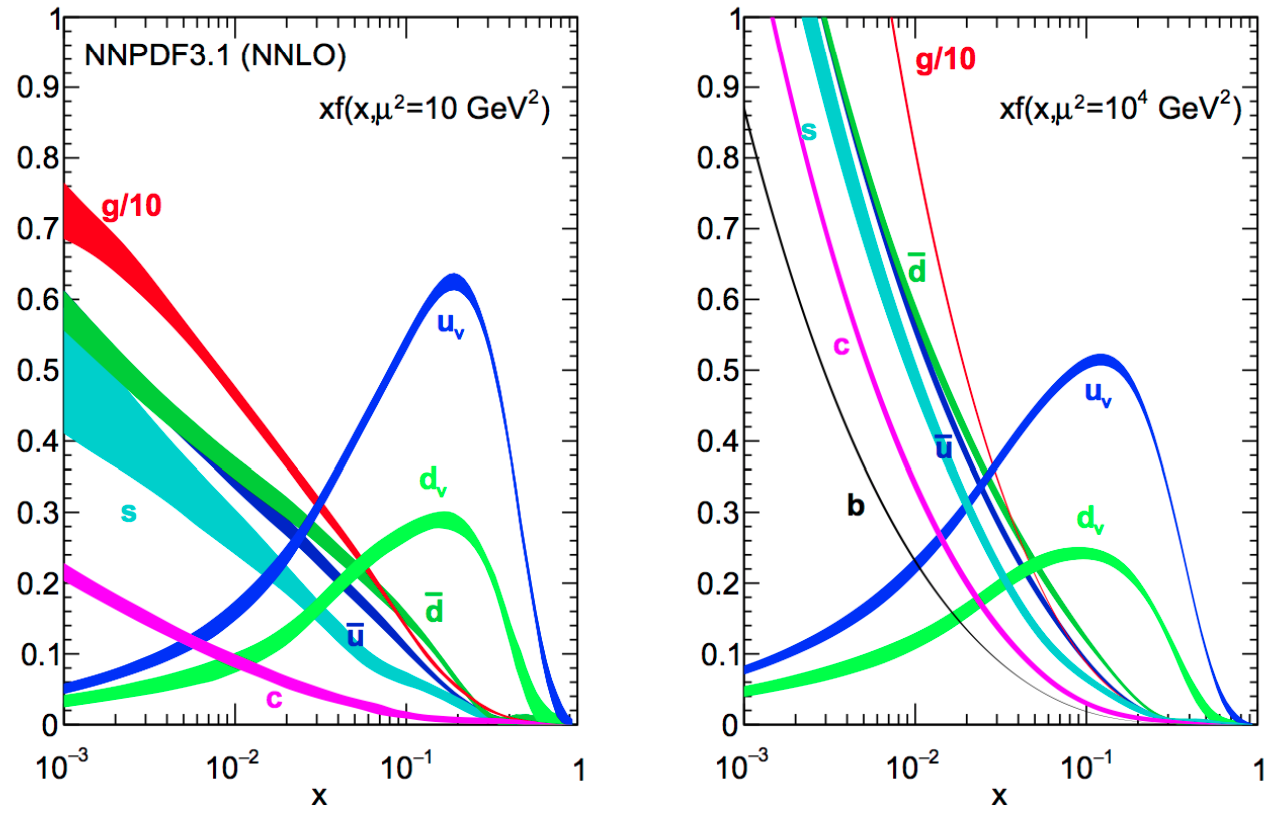
\includegraphics[width=0.9\textwidth]{Figures/PDF}
	\caption[The parton distribution function of the proton scaled by the fraction of momentum carried by the parton, $xf(x, \mu^2)$ with respect to the fraction of momentum carried by the parton. The left panel shows the distributions with respect to a lower energy scale and the right panel with respect to a higher energy scale.]{ The parton distribution function of the proton scaled by the fraction of momentum carried by the parton, $xf(x, \mu^2)$ with respect to the fraction of momentum carried by the parton. The left panel shows the distributions with respect to a lower energy scale and the right panel with respect to a higher energy scale~\cite{NNPDF3p1}. }
	\label{fig:pdf}
\end{figure}

The prediction of the inclusive \ttbar{} cross section from proton-proton collisions is shown in Fig.~\ref{fig:incttbar}, together with current experimental measurements. 
The prediction from proton-anti-proton collisions is also shown.
The cross sections converge at higher energies due to the increase in collisions between non-valence partons the distribution of which is identical in protons and anti-protons.
At \com{}, the inclusive \ttbar{} production cross section was calculated to be $831.8^{+19.8}_{-29.2}(\text{scale})\pm35.1(\text{PDF}+\alpS)\pb$~\cite{TOPpp}.
This \ttbar{} cross section is calculated to next-to-next-to-leading-order (\NNLO{}) accuracy in perturbative \QCD{}, including resummation of next-to-next-to-leading logarithmic soft-gluon terms with \textsc{Top++} (v2.0)~\cite{Th:XSEC1,Th:XSEC2,Th:XSEC3,Th:XSEC4,Th:XSEC5,Th:XSEC6,Th:XSEC7}.
% TODO ADD MORE?
% The scale uncertainty in this \ttbar{} cross section comes from the independent variation of the factorization and renormalization scales.
\begin{figure}[htpb]
	\centering
	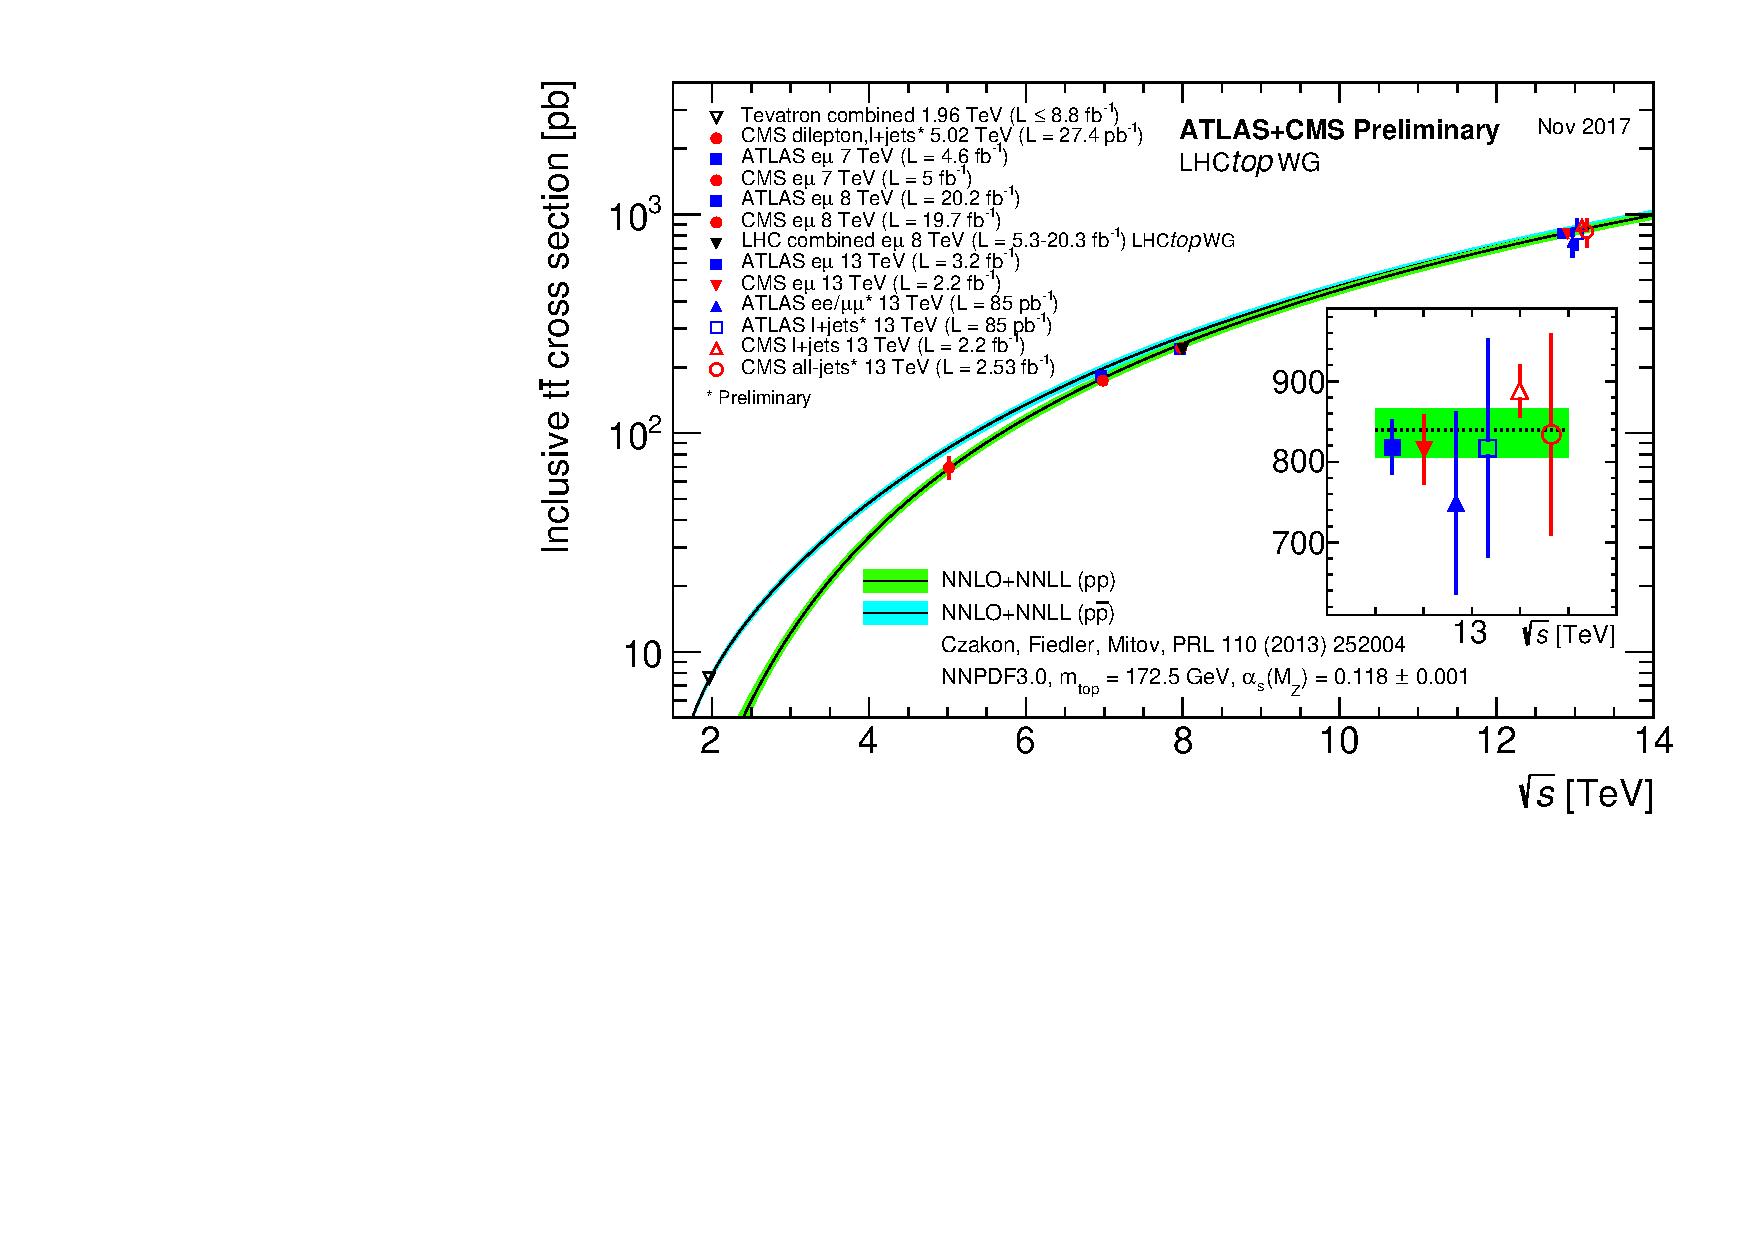
\includegraphics[width=0.9\textwidth]{Figures/tt_curve_sqrts_cms}
	\caption[The inclusive \ttbar cross section, measured by ATLAS, CMS and the Tevatron in different decay channels at multiple \sqrts{}. Also shown is the most precise theoretical prediction to date.]{ The inclusive \ttbar cross section, measured by ATLAS, CMS and the Tevatron in different decay channels at multiple \sqrts{}. Also shown is the most precise theoretical prediction to date~\cite{LHCTopWG_Plots}. }
	\label{fig:incttbar}
\end{figure}
% subsection top_quark_production (end)

\subsection{Order of perturbation} % (fold)
\label{sub:order_of_perturbation}

The cross section of a process depends on a quantity known as the \textit{matrix element}
\begin{equation*}
	\hat{\sigma}_{\ttbar{}}\propto\abs{\mathcal{M}}^2
\end{equation*}
and the matrix element can be calculated using the Feynman rules from Feynman diagrams.
Increasing the order of perturbation essentially adds an additional parton to each diagram which makes the matrix-element calculation much more complex but gives increasing accuracy.
A comparison of the Feynman diagrams at leading order (\LO{}) and next-to-leading order (\NLO{}) is shown in Fig.~\ref{fig:feyn-nlo}, where in the top left panel a simple \LO{} tree-diagram is shown. 
The top right panel shows loops in the propagator which can be related to the running of \alpS{}.
The rest of the panels show \NLO{} processes, where the centre two panels are displaying loops corresponding to virtual particles 
% whose properties counteract the infra-red divergences introduced by the radiation of soft collinear partons of the form seen in the lower two panels.
and the lower two panels contribute real partons to the final state.
\begin{figure}
\centering
\begin{resizedtikzpicture}{0.45\linewidth}
\begin{feynman}
	\vertex (A);
	\vertex [below=3cm of A](B);
	\vertex [below right=1.5cm and 3cm of A](C);

	\vertex [right=1cm of C](D1);
	\vertex [right=2cm of C](D2);
	\vertex [right=3cm of C](D3);
	\vertex [above right=0.375cm and 0.75cm of D3] (E1);
	\vertex [above right=0.75cm and 1.5cm of D3] (E2);
	\vertex [above right=1.5cm and 3cm of D3] (E3);
	\vertex [above right=0.375cm and 0.75cm of D3] (F1);
	\vertex [below right=0.75cm and 1.5cm of D3] (F2);
	\vertex [below right=1.5cm and 3cm of D3] (F3);

	\diagram* {
	(A) -- [fermion] (C),
	(B) -- [anti fermion] (C),

	(C) -- [gluon] (D3),
	(D3) -- [fermion] (E3),
	(D3) -- [anti fermion] (F3),
	};
\end{feynman}
\end{resizedtikzpicture} \\
\caption[A Feynman diagram showing a \LO{} process.]{A Feynman diagram showing a \LO{} process.}
\label{fig:feyn-nlo1}
\end{figure}

\begin{figure}
\centering
\begin{resizedtikzpicture}{0.45\linewidth}
\begin{feynman}
	\vertex (A);
	\vertex [below=3cm of A](B);
	\vertex [below right=1.5cm and 3cm of A](C);

	\vertex [right=1cm of C](D1);
	\vertex [right=2cm of C](D2);
	\vertex [right=3cm of C](D3);
	\vertex [above right=0.375cm and 0.75cm of D3] (E1);
	\vertex [above right=0.75cm and 1.5cm of D3] (E2);
	\vertex [above right=1.5cm and 3cm of D3] (E3);
	\vertex [above right=0.375cm and 0.75cm of D3] (F1);
	\vertex [below right=0.75cm and 1.5cm of D3] (F2);
	\vertex [below right=1.5cm and 3cm of D3] (F3);

	\diagram* {
	(A) -- [fermion] (C),
	(B) -- [anti fermion] (C),

	(C) -- [gluon] (D3),
	(D3) -- [fermion] (E3),
	(D3) -- [anti fermion] (F3),
	(D2) -- [gluon, half left] (E1),
	};
\end{feynman}
\end{resizedtikzpicture}
\hspace{1cm}
\begin{resizedtikzpicture}{0.45\linewidth}
\begin{feynman}
	\vertex (A);
	\vertex [below=3cm of A](B);
	\vertex [below right=1.5cm and 3cm of A](C);

	\vertex [right=1cm of C](D1);
	\vertex [right=2cm of C](D2);
	\vertex [right=3cm of C](D3);
	\vertex [above right=0.375cm and 0.75cm of D3] (E1);
	\vertex [above right=0.75cm and 1.5cm of D3] (E2);
	\vertex [above right=1.5cm and 3cm of D3] (E3);
	\vertex [above right=0.375cm and 0.75cm of D3] (F1);
	\vertex [below right=0.75cm and 1.5cm of D3] (F2);
	\vertex [below right=1.5cm and 3cm of D3] (F3);

	\diagram* {
	(A) -- [fermion] (C),
	(B) -- [anti fermion] (C),

	(C) -- [gluon] (D3),
	(D3) -- [fermion] (E3),
	(D3) -- [anti fermion] (F3),
	(E2) -- [gluon, half left] (F2),
	};
\end{feynman}
\end{resizedtikzpicture} \\
\vspace{0.5cm}
\begin{resizedtikzpicture}{0.45\linewidth}
\begin{feynman}
	\vertex (A);
	\vertex [below=3cm of A](B);
	\vertex [below right=1.5cm and 3cm of A](C);
	\vertex [below right=0.75cm and 1.5cm of A](A1);
	\vertex [above right=0.75cm and 1.5cm of A1](A2);

	\vertex [right=1cm of C](D1);
	\vertex [right=2cm of C](D2);
	\vertex [right=3cm of C](D3);
	\vertex [above right=0.375cm and 0.75cm of D3] (E1);
	\vertex [above right=0.75cm and 1.5cm of D3] (E2);
	\vertex [above right=1.5cm and 3cm of D3] (E3);
	\vertex [above right=0.375cm and 0.75cm of D3] (F1);
	\vertex [below right=0.75cm and 1.5cm of D3] (F2);
	\vertex [below right=1.5cm and 3cm of D3] (F3);
	\vertex [below right=0.75cm and 1.5cm of E2] (G);

	\diagram* {
	(A) -- [fermion] (C),
	(B) -- [anti fermion] (C),

	(C) -- [gluon] (D1),
	(D1) -- [gluon, half left] (D2),
	(D2) -- [gluon, half left] (D1),
	(D2) -- [gluon] (D3),
	(D3) -- [fermion] (E3),
	(D3) -- [anti fermion] (F3),
	};
\end{feynman}
\end{resizedtikzpicture} \\
\caption[A set of Feynman diagrams showing virtual \NLO processes. These loops are responsible for the running of the strong coupling constant.]{A set of Feynman diagrams showing virtual \NLO processes. These loops are responsible for the running of the strong coupling constant.}
\label{fig:feyn-nlo2}
\end{figure}

\begin{figure}
\centering
\begin{resizedtikzpicture}{0.45\linewidth}
\begin{feynman}
	\vertex (A);
	\vertex [below=3cm of A](B);
	\vertex [below right=1.5cm and 3cm of A](C);
	\vertex [below right=0.75cm and 1.5cm of A](A1);
	\vertex [above right=0.75cm and 1.5cm of A1](A2);

	\vertex [right=1cm of C](D1);
	\vertex [right=2cm of C](D2);
	\vertex [right=3cm of C](D3);
	\vertex [above right=0.375cm and 0.75cm of D3] (E1);
	\vertex [above right=0.75cm and 1.5cm of D3] (E2);
	\vertex [above right=1.5cm and 3cm of D3] (E3);
	\vertex [above right=0.375cm and 0.75cm of D3] (F1);
	\vertex [below right=0.75cm and 1.5cm of D3] (F2);
	\vertex [below right=1.5cm and 3cm of D3] (F3);

	\diagram* {
	(A) -- [fermion] (C),
	(B) -- [anti fermion] (C),

	(C) -- [gluon] (D3),
	(D3) -- [fermion] (E3),
	(D3) -- [anti fermion] (F3),
	(A1) -- [gluon] (A2),
	};
\end{feynman}
\end{resizedtikzpicture}
\hspace{1cm}
\begin{resizedtikzpicture}{0.45\linewidth}
\begin{feynman}
	\vertex (A);
	\vertex [below=3cm of A](B);
	\vertex [below right=1.5cm and 3cm of A](C);
	\vertex [below right=0.75cm and 1.5cm of A](A1);
	\vertex [above right=0.75cm and 1.5cm of A1](A2);

	\vertex [right=1cm of C](D1);
	\vertex [right=2cm of C](D2);
	\vertex [right=3cm of C](D3);
	\vertex [above right=0.375cm and 0.75cm of D3] (E1);
	\vertex [above right=0.75cm and 1.5cm of D3] (E2);
	\vertex [above right=1.5cm and 3cm of D3] (E3);
	\vertex [above right=0.375cm and 0.75cm of D3] (F1);
	\vertex [below right=0.75cm and 1.5cm of D3] (F2);
	\vertex [below right=1.5cm and 3cm of D3] (F3);
	\vertex [below right=0.75cm and 1.5cm of E2] (G);

	\diagram* {
	(A) -- [fermion] (C),
	(B) -- [anti fermion] (C),

	(C) -- [gluon] (D3),
	(D3) -- [fermion] (E3),
	(D3) -- [anti fermion] (F3),
	(E2) -- [gluon] (G),
	};
\end{feynman}
\end{resizedtikzpicture} \\
\caption[A set of Feynman diagrams showing real \NLO{} processes. These are represented by the emission of real additional partons that can be seen in the final state.]{A set of Feynman diagrams showing real \NLO{} processes. These are represented by the emission of real additional partons that can be seen in the final state.}
\label{fig:feyn-nlo3}
\end{figure}
% \caption[A set of Feynman diagrams showing \LO{} and \NLO{} processes. In the top left panel, the leading order diagram is shown. The top right panel shows a gluon-loop in the propagator. These loops are responsible for the running strong coupling constant. The two middle panels show \NLO loops providing virtual particles to the diagrams and corrections in the renormalisation scale. Finally, the bottom two panels show the real additional partons that can be seen in the final state due to \NLO{} matrix-element calculations.]{A set of Feynman diagrams showing \LO{} and \NLO{} processes. In the top left panel, the leading order diagram is shown. The top right panel shows a gluon-loop in the propagator. These loops are responsible for the running strong coupling constant. The two middle panels show \NLO loops providing virtual particles to the diagrams and corrections in the renormalisation scale. Finally, the bottom two panels show the real additional partons that can be seen in the final state due to \NLO{} matrix-element calculations.}

Perturbation theory is valid at high energy scales, however at lower energy scales \QCD{} production becomes non-perturbative and the cross section is not able to be calculated using the matrix-element.
The method of dealing with non-perturbative \QCD{} is dealt with in Sec.~\ref{sec:additional_interactions_and_soft_processes}.

% Perturbation theory is valid at high energy scales, however when calculating including contributions at a much softer scale, see Section TODO, \alpS{} is accompanied by large logarithms of the ratio of the two scales.
% When approaching the edge of phase space close to the lower energy scale, such that the real emissions from soft gluons are neglected, but the virtual contributions still exist, these large logarithms are no longer cancelled.
% This leads to divergences in the partonic cross section in this area of phase space and so a soft gluon resummation must be applied.

% subsection order_of_perturbation (end)


\subsection{Top quark decay} % (fold)
\label{sub:top_quark_decay}

In the \SM{}, the top quark will decay 99.9\%~\cite{PDG} of the time to a \bquark{} quark and \Wboson{} boson.
The \Wboson{} boson then subsequently decays either into a \qpqbar{} pair (hadronic) or a \lepton{}\neutrinobar{} pair (leptonic).
In the case of \ttbar{} production, this leads to three classes of final states, the first where both \Wboson{} bosons decay leptonically, the second where both decay  hadronically and lastly where one decays leptonically and the other hadronically.
These are known as the \textit{dilepton}, \textit{all-hadronic} and \textit{single lepton} decay channels respectively.
The probability of decaying to a specific final state (\textit{branching ratio}) is approximately $10\%$ for the dilepton channel and $45\%$ for the hadronic and single lepton channels.
% W->(ud*3, cs*3, enu, munu, taunu) us cd suppressed

Each final state category has merits and drawbacks for use in analyses. 
The dilepton final state provides the most clean experimental signature, however this comes at the cost of a reduced branching ratio.
It is difficult to fully reconstruct the whole event as both neutrinos contribute to the missing transverse momentum.
The all-hadronic final state in comparison has a large branching ratio and a large multijet \QCD{} background.
The high jet multiplicity can also cause problems from the combinatorics when reconstructing the \ttbar{} system.
While the all-hadronic final state is difficult at lower collision energies, it gains in sensitivity when analysed at high collision energies.
This is because the decay products of the top quark collimate and merge into a single jet, which is able to be tagged as coming from a top quark, through jet-substructure techniques.
Finally the single lepton decay channel has a large branching ratio, but with much reduced backgrounds with respect to the all-hadronic final state. 
The final states in which a tau particle is produced are often neglected however, due to the added complexity of reconstructing them.
More details about the reconstruction of particles can be found in Ch.~\ref{ch:ObjectReconstruction}.
% For this reason \lepton{} will be used to refer to just \electron{} and \muon{}.
% subsection tt_decay (end)

\subsection{Top quark cross section measurements} % (fold)
\label{sub:top_quark_cross_section_measurements}

Figure.~\ref{fig:incttbar} shows, in addition to the theoretical prediction of the inclusive \ttbar{} production cross section, the corresponding experimental measurements, from both the CMS and A Toriodal Large ApparatuS (ATLAS) at different centre-of-mass energies (\sqrts{}) in all of the channels previously stated.
At CMS, the inclusive \ttbar{} cross section measurements are performed at 13\TeV{}~\cite{TOP16005, TOP16006} at 7 and 8 \TeV{}~\cite{TOP10001, TOP10002, TOP10003, TOP11002, TOP11003, TOP11004, TOP11005, TOP12007, TOP12026, TOP12041, TOP13004, TOP14018} and at 5\TeV{}~\cite{TOP16023}.
Inclusive cross section measurements have been performed for \ttbar{} production in association with a photon~\cite{TOP14008}, vector boson~\cite{TOP17005} and most recently \Hboson{} boson~\cite{HIG17035}.

Measurements of the \ttbar{} production cross section with respect to some other variable are known as \textit{differential} cross section measurements.
Differential cross section measurements are especially useful for testing the understanding of state-of-the-art theoretical models.
Ideally, these models should describe \ttbar{} production with respect to all kinematic variables accurately, including contributions from additional jets, and should do so for all \sqrts{}.
In practice this is not the case, with the \ttbar{} models being \textit{tuned} to best describe the kinematic distributions.
A tune is a complete set of simulation parameters describing physics processes within the simulation of the model, which have been varied to best describe differential data distributions.
Figure.~\ref{fig:8TeVTuning} shows the effect of this tuning on a set of \ttbar{} models, where the new tune is shown in solid and the old in dashed, when comparing the cross sections as a function of the magnitude of the transverse momentum of the hadronically decaying top quark, \ptToph{}, and the additional jet multiplicity.
It is worth noting, that a tune applied to a specific model may not describe the differential data better than when applied to another independent model.
The different models behind \ttbar{} production are explained in more detail in Ch.~\ref{ch:MC}.
Indeed by changing the tune, it may cause the same model to describe some kinematic distributions to a worse degree, while improving other parts of the phase space.
\begin{figure}[htpb]
	\centering
	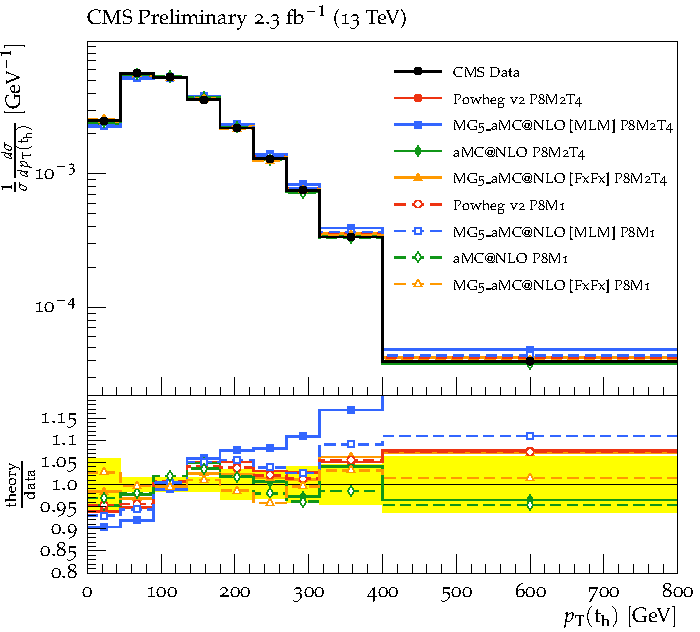
\includegraphics[width=0.49\textwidth]{Figures/TuningEx3}
	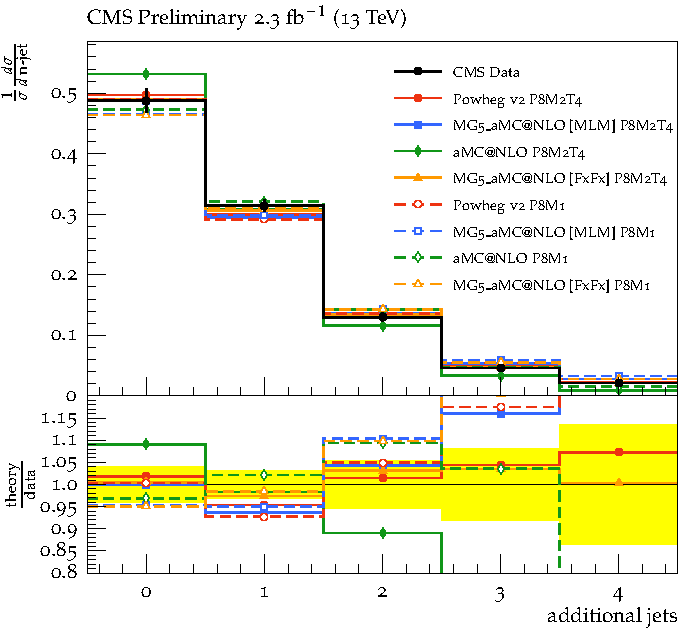
\includegraphics[width=0.49\textwidth]{Figures/TuningEx2}
	\caption[Comparison of different \ttbar{} models with the old \CUETold{} tune, represented by dashed lines, and the new \CUET{} tune, given by solid lines. The left panel shows the comparison for the distribution of the \pt{} of the hadronically decaying top quark and the right panel for the additional jets distribution.]{ Comparison of different \ttbar{} models with the old \CUETold{} tune, represented by dashed lines, and the new \CUET{} tune, given by solid lines. The left panel shows the comparison for the distribution of the \pt{} of the hadronically decaying top quark and the right panel for the additional jets distribution~\cite{Gen:CUETP8M2T4}. }
	\label{fig:8TeVTuning}
\end{figure}

Differential top quark cross section measurements can be presented to \textit{particle level} where the kinematic distributions are constructed with respect to stable particles in the detector (mean lifetime longer than 30\ps{}).
Alternatively, they can be presented to \textit{parton level}, where the results are extrapolated with respect to the final state partons or to \textit{detector level}, where no extrapolation is performed.
Similarly, the results can be presented in a phase space similar to that accessible by the detector, the \textit{visible phase space} or extrapolated to the \textit{full phase space}.
Measurements that are presented to parton level or that are extrapolated to the full phase space are influenced by large theoretical uncertainties due to that extrapolation and as such most analyses present measurements to particle level in the visible phase space.
All the \ttbar{} cross section measurements performed by the CMS (and ATLAS) experiment are completely complementary to each other and are presented at 7 and 8\TeV{}~\cite{TOP11013,TOP12028,TOP14012,TOP14013} and at 13\TeV~\cite{TOP15013, TOP16007,TOP16008,TOP16010,TOP17002}.

This thesis looks at differential cross section measurements as a function of kinematic event variables in the single lepton channel presented to particle level in a visible phase space.
The kinematic event variables are variables that do not require the reconstruction of the complete \ttbar{} system.
The event variables considered are the jet multiplicity, \NJET{}, the scalar sum of the jet \pt{}, \HT{}, the scalar sum of the \pt{} of all particles, \ST{}, the magnitudes of the transverse momentum imbalance, \ptmiss{}, the \pt{} of the leptonically decaying \Wboson{} boson, \WPT{}, the \pt{} of the lepton, \LPT{} and lepton pseudorapidity \LETA{}.
These event variables are defined in Sec.~\ref{sec:var}.
Measurements with respect to kinematic event variables have been performed at 7 and 8\TeV{}~\cite{TOP12042} and 13\TeV{} with a much smaller data set~\cite{TOP16014}.
% subsection top_quark_cross_section_measurements (end)

% \subsection{TODO} % (fold)
% \label{sub:why_top_physics_is_interesting}
% \begin{itemize}
% 	\item TODO: ALL THE REFERENCES.
% 	\item TODO: TOP TAGGING REFERENCE
% 	% \item TODO: DIFFERENTIATE BETWEEN FIELD AND FIELD STRENGTH TENSOR.
% 	\item TODO: INTRODUCE RIVET HERE?
% 	\item TODO: LO, NLO, NNLO OR IN SIM CHAPTER?
% 	\item TODO: ADD ATLAS REFERENCES? (MAYBE TO MANY HERE?)
% 	\item TODO: BACKGROUND FEYNMANS
% \end{itemize}




